\begin{comment}

\section{Introdução}
Neste capítulo, a arquitetura do sistema é apresentada, incluindo seus módulos e tecnologias de apoio que foram utilizadas no desenvolvimento da aplicação.
Nesta seção, o autor apresenta o projeto da sua contribuição. Quando se trata de desenvolvimento de um software é recomendado que nesta seção o autor apresente a arquitetura do sistema, composta de: a) arquitetura em si (camadas que compõe o sistema); b) principais diagramas da Engenharia de Software que sintetizam o projeto, e; c) tecnologias de apoio usadas no desenvolvimento do software.
Outros modelos de trabalho podem apresentar nesta seção a metodologia, a técnica e os instrumentos de análise e comparação. A fundamentação científica é fundamental para subsidiar a construção destas contribuições.   


\section{Tecnologias de Apoio}


\subsection{\textit{Tecnologia 1}}
...

\subsection{\textit{Tecnologia 2}}
...

\section{Arquitetura}




\begin{figure}[htp]
\centering
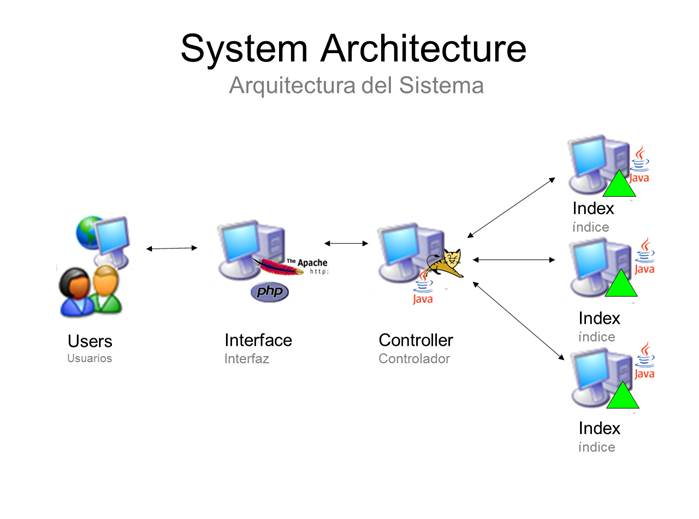
\includegraphics[scale=0.8]{img/ArquiteturaSistema.jpg}
\caption[Arquitetura do Sistema]{Arquitetura do Sistema}
\label{arquituraGeral}
\end{figure}



\subsection{Users}
...
\subsection{Interface}
...
\subsection{Controller}
...

\section{Considerações Finais}

\end{comment}

Na \autoref{sec:metodo} serão descrito os passos que serão realizados, os processos metodológicos adotados na pesquisa e como ocorrerá cada etapa do projeto. Já na \autoref{sec:estudo} serão abordados os elementos essenciais de um estudo de caso e a descrição de como será realizado o estudo de caso deste projeto de pesquisa. E, por fim, na \autoref{sec:classif} será realizado a classificação do projeto de pesquisa quanto aos gêneros identificados.

\section{Descrição do processo metodológico} \label{sec:metodo}

Nesta seção serão descritos os processos que serão realizados para se alcançar os objetivos geral e específicos estabelecidos. Na \autoref{fig:processo} serão ilustrados os passos básicos do processo feito para a aplicação deste projeto de pesquisa, contendo as fontes de dados, os passos e os resultado que serão gerados.

\subsection{Coleta de Dados}
Para este projeto de pesquisa, serão adotadas 4 fontes de dados. Esses dados coletados darão suporte para proposições que serão feitas para solucionar o problema. As quatro fontes de dados que serão usadas são: as respostas do Kahoot! de 2018.2, os resultados finais do processo de avaliação somativa de 2018.2, as respostas do Kahoot! de 2019.2 e os resultados parciais de 2019.2, as quatro na disciplina de Interface Humano-Computador.

\subsubsection{Respostas ao Kahoot!}
O Kahoot! é uma plataforma de GBL e foi descrita melhor na \autoref{sec:Kahoot!}. Na disciplina de Interface Humano-Computador (IHC), ela foi utilizada em 2018.2 e será utilizada em 2019.2 novamente. O Kahoot! tem um caráter fortemente formativo, sendo aplicado ao final de cada aula, com questões elaboradas pelo professor que abordem assuntos que foram ministrados na aula. 

As perguntas são de múltipla-escolha, tendo entre duas e cinco alternativas de respostas para o aluno. Neste projeto de pesquisa, serão usados os dados provenientes de respostas dadas pelos alunos aos questionários aplicados nas turmas de 2018.2 e 2019.2 da disciplina de Interface Humano-Computador da UFG, localizada em Jataí, sudoeste goiano. Na \autoref{fig:kahoot} é apresentado um \textit{Screenshot} de um exemplo de pergunta no Kahoot!

\subsubsection{Resultados parciais e finais da Avaliação Somativa}

O processo de Avaliação Somativa foi descrito na \autoref{sec:AvaSom}. O Kahoot! além de caráter formativo, ele também tem, ainda que pouco, caráter somativo. Além disso, serão utilizadas os resultados parciais e finais da disciplina de IHC para a analise dos resultados do projeto.

Da turma de 2018.2, serão usados os resultados finais da Avaliação Somativa, sendo que a disciplina já se encerrou, tendo apenas que coletar esses dados que estão armazenados. Já na turma de 2019.2, os resultados da Avaliação Somativa que serão usados são os parciais, consistindo de 2/3 da disciplina já realizada. O motivo desse ocorrido se dá em função do período que será necessário para obtenção e análise destes, visto que para se ter os resultados finais não haveria tempo hábil para realizar a análise completa destes, tendo assim uma perda. Acredita-se que, com esta porção de dados, será suficiente se ter resultados significativos e, assim, apresentar uma contribuição científica relevante.

\begin{figure}
    \centering
    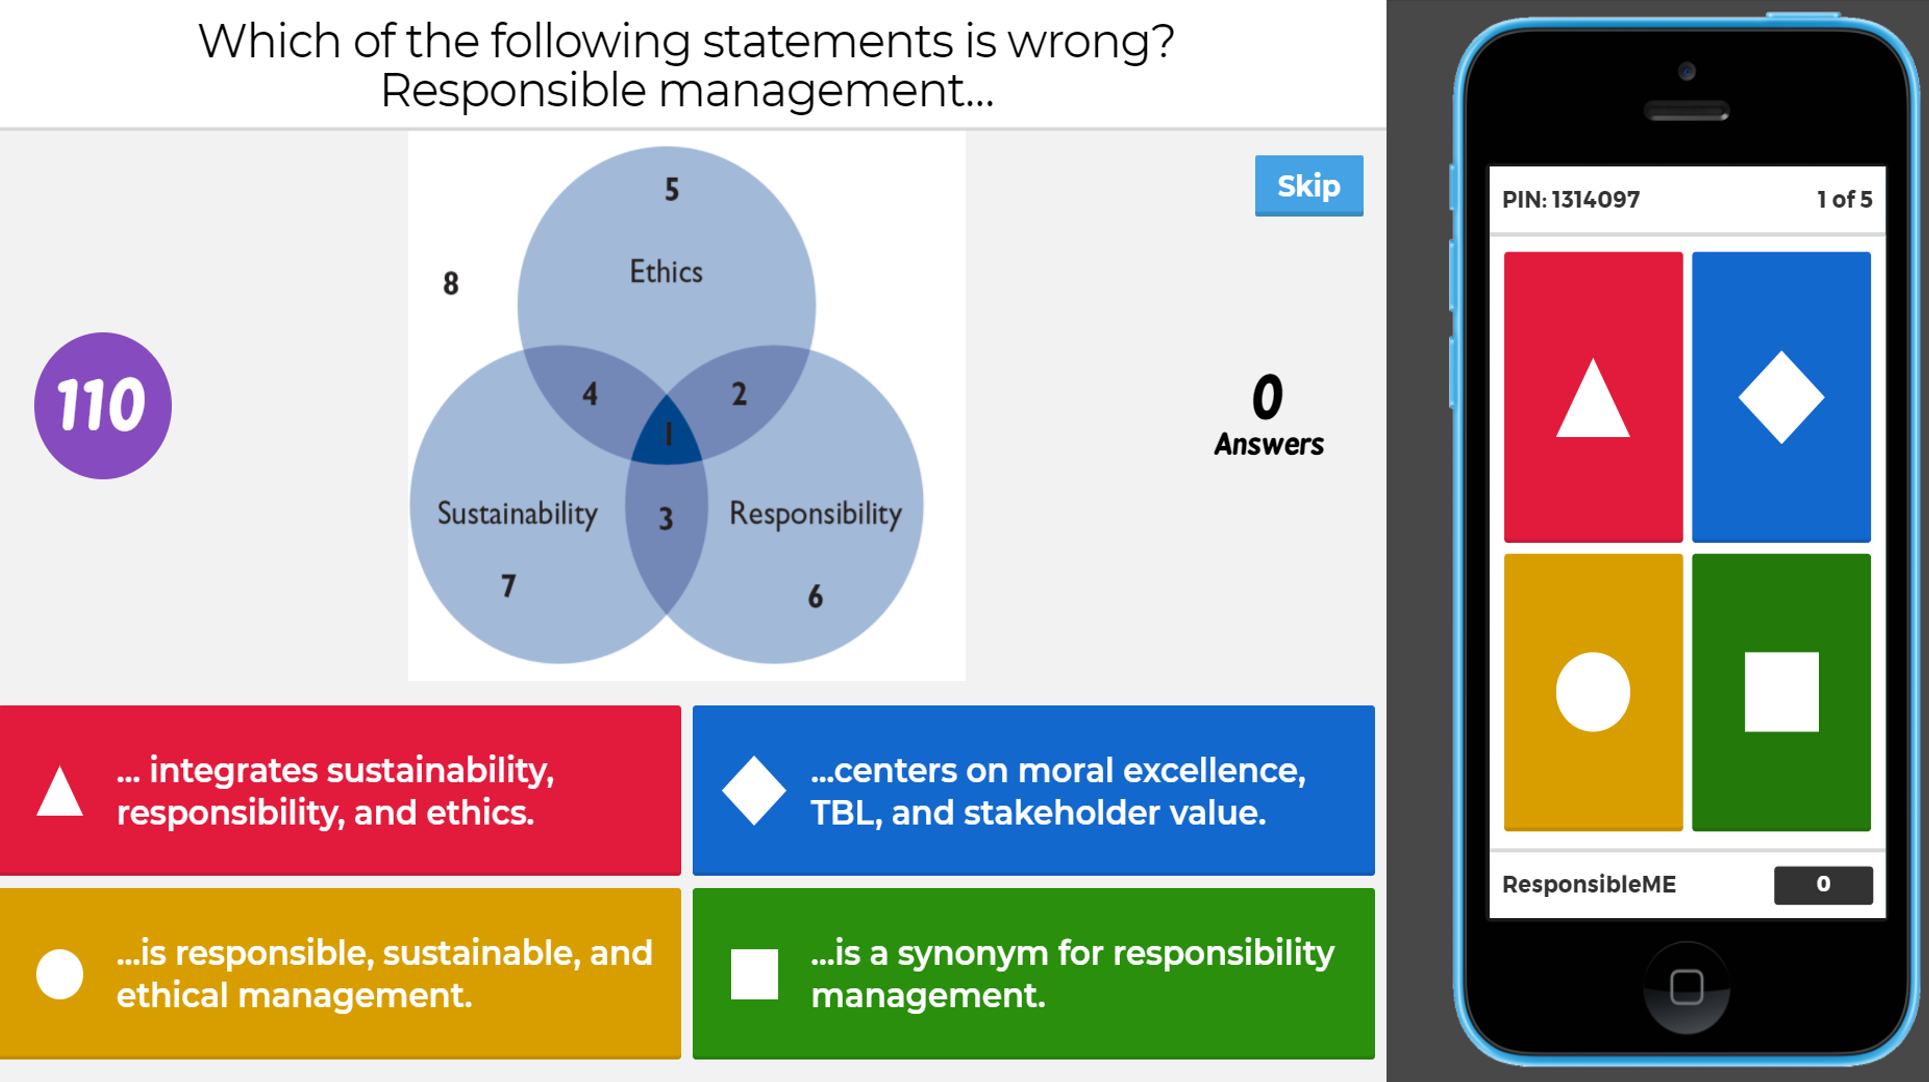
\includegraphics[width=0.7\textwidth]{modelo-monografia-rej-2018/img/KahootScreenshot.png}
    \caption{Exemplo de uma questão feita no Kahoot!}
    \label{fig:kahoot}
\end{figure}
 
\subsection{Projeto e Implementação da Rede Neural}

O projeto da Rede consiste em pegar um conjunto de dados de entrada, aplicar essa entrada em neurônios, onde esses reajustarão os pesos destas. A rede produz uma saída com a ``previsão'' da rede, aprovado ou reprovado --- sendo depois indicado o grau, provavelmente ou fortemente. O conjunto de entrada da Rede é composto por um vetor onde estarão as respostas dadas pelos alunos.

A Rede Neural Artificial será a técnica de aprendizagem de máquina usada por este projeto de pesquisa. A descrição desta foi feita na \autoref{sec:RNA}. Para isso, será projetada uma Rede Neural Artificial, adotando uma arquitetura de rede especifica.

A implementação da rede será feita na linguagem de programação \textit{Python}, que é uma linguagem interpretada, de \textit{script}, imperativa, orientada a objetos, funcional, de tipagem dinâmica e forte. Python é uma das opções mais comuns, quando se trata de Inteligência Artificial, talvez a que tenha mais biblioteca para Aprendizado de Máquina e Análise de Dados.

Uma destas bibliotecas é a TensorFlow, que é de código-aberto. É com ela que será criada e treinada a Rede Neural proposta por esta pesquisa. Essa biblioteca consiste em detectar e decifrar padrões e correlações, análogo à maneira com que o seres-humanos aprendem e raciocinam. 

{\color{red} [Por quê Python e TensorFlow?]}

\subsection{Treinamento da Rede Neural}

Como dito, o treinamento da Rede Neural será feito com a biblioteca TensorFlow na linguagem Python. Os dados usados para esse treinamento da rede serão os coletados das turmas de 2018.2 e 2019.2 de IHC. O projeto consiste em dividir as resposta pelo período em que elas foram aplicadas, sendo estes em 3 subdivisões.

A primeira rede será a rede com as entradas de dados dos primeiros 15 dias de aula, sendo estas entradas as respostas dadas nesse período às questões do Kahoot!, a segunda divisão será feita da mesma forma, porém as entradas serão as respostas dos primeiros 30 dias de aula. E, por fim, a última rede consistirá das respostas dadas nos primeiros 60 dias de aula.

Para melhor elucidação das arquiteturas, foram feitas 3 figuras para representar as redes que serão criadas, onde estão ilustradas como serão feitas as redes, e os conjuntos de entradas que serão adotadas. Na primeira rede (Ver \autoref{fig:rede01}), o conjunto de entrada será de 40 questões, sendo 10 por aula e 4 aulas no período de 15 dias. Na segunda rede (Ver \autoref{fig:rede02}), serão 30 dias e, consequentemente, o dobro de questões. E na terceira rede (Ver \autoref{fig:rede03}), o mesmo. Serão 160 questões em um período de 60 dias.

\begin{figure}
    \centering
    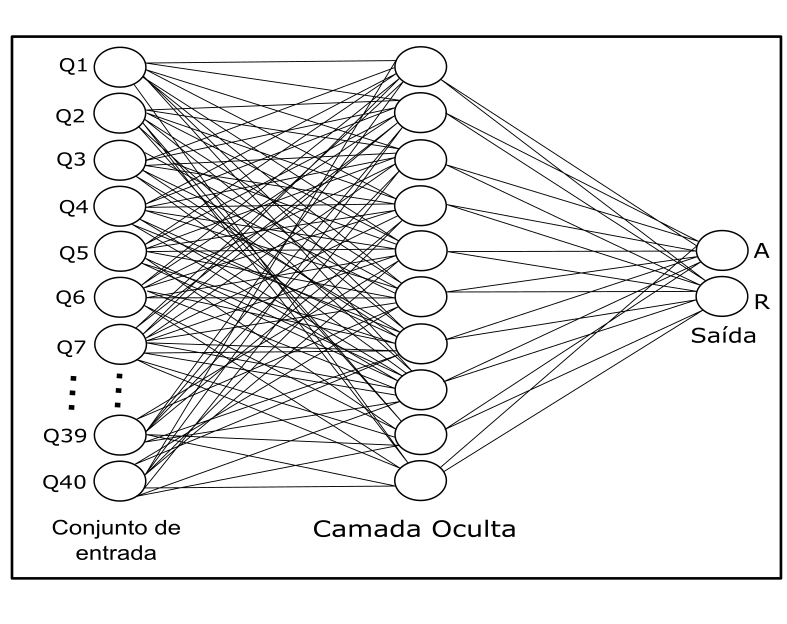
\includegraphics[width=0.9\textwidth]{modelo-monografia-rej-2018/img/rede01_15.png}
    \caption{Rede 01 - 15 dias de respostas}
    \label{fig:rede01}
\end{figure}

\begin{figure}
    \centering
    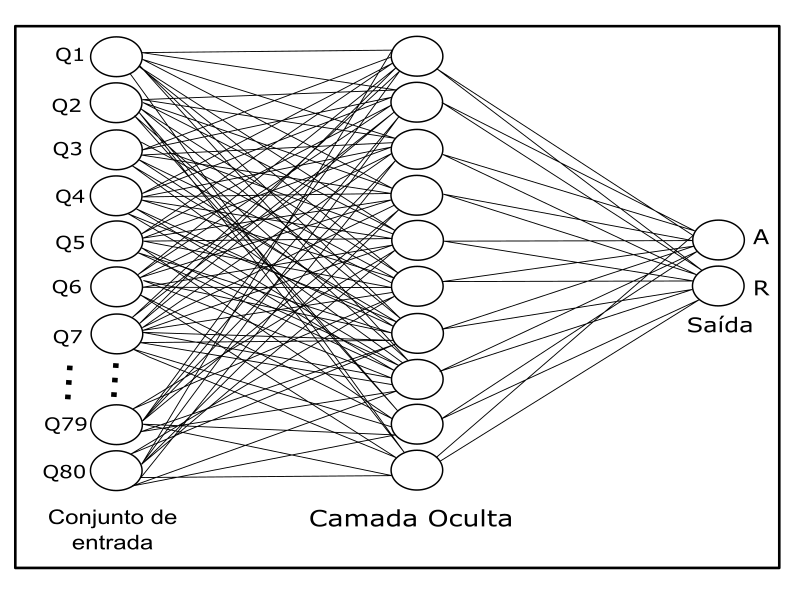
\includegraphics[width=0.9\textwidth]{modelo-monografia-rej-2018/img/rede02_30.png}
    \caption{Rede 02 - 30 dias de respostas}
    \label{fig:rede02}
\end{figure}

\begin{figure}
    \centering
    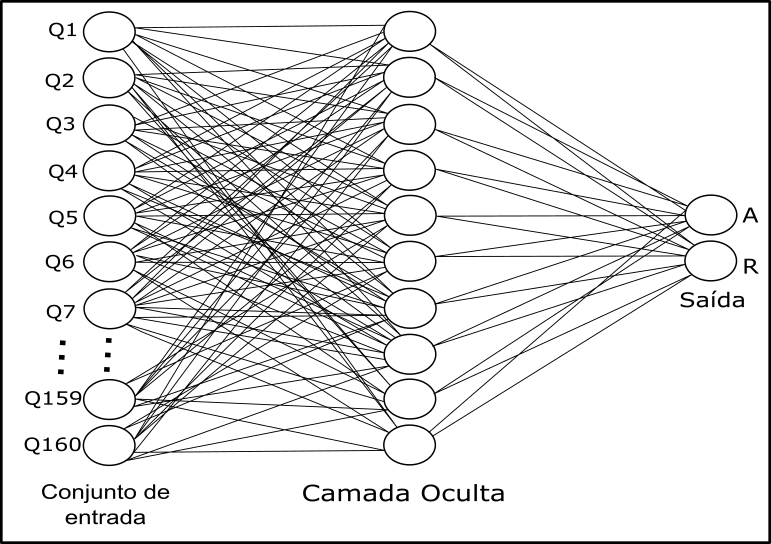
\includegraphics[width=0.9\textwidth]{modelo-monografia-rej-2018/img/rede03_60.png}
    \caption{Rede 03 - 60 dias de respostas}
    \label{fig:rede03}
\end{figure}

\subsection{Teste e Validação}

O teste e a validação serão feitos nas semanas subsequentes às estabelecidas para o treinamento, com as redes já com os ``neurônios'' com seu respectivo peso, feito através do processo de treino da rede. Ao fazer o teste e a validação, os alunos serão classificados em 4 grupos, que apresentarão o grau de risco e a situação dos alunos frente às previsões realizadas pela rede.

Serão usadas as respostas dos alunos ao Kahoot!. A rede fará a análise dos dados e verificará se há um padrão entre estes dados, se há uma correlação e, ao fazer as ligações ``sinápticas'' artificiais, como uma reprodução --- ou simulação --- do processo de raciocínio humano fará inferências quanto ao resultado acadêmico no processo de avaliação somativa, produzindo assim uma classificação deste aluno.

\subsection{Classificação dos alunos}
Após a análise ser feita pela Rede, o conjunto de saída apontará o aluno para que este integre um entre quatro grupos que serão estabelecidos. Os grupos seriam definidos como: Fortemente Reprovados (FR), Provavelmente Reprovados (PR), Provavelmente Aprovados (PA) e Fortemente Aprovados (FA). Esses níveis dizem respeito ao quão o aluno está propenso à reprovar. Pensando em um plano cartesiano, seria como se no eixo das abcissas fosse posto esses níveis classificatórios. Nessa analogia, quanto mais à esquerda o aluno fosse classificado, maior seria a chance do aluno ser reprovado na disciplina, quanto mais à direita o aluno fosse classificado, maior seria a chance desse aluno ser aprovado.

A questão que aparece ao se fazer essa classificação é a seguinte: ``Um aluno não pode ser classificado de forma errada?''. Sim, ele pode, e isso é descrito por quatro conceitos (ver \autoref{fig:Venn}) importantes de serem definidos neste projeto de pesquisa, que são:

\begin{itemize}
    \item \textbf{Falsos-negativos (FN)}: Com os resultados alcançados pela rede, alunos podem ser classificados como se não estivessem no grupo de risco de reprovação, mas acabam reprovando. São os chamados falsos-negativos.
    \item \textbf{Falsos-positivos (FP)}: Os alunos podem ainda ser classificados como alunos em situação de risco de reprovação, mas ao final da disciplina alguns desses alunos serem aprovados, constatando assim os chamados Falsos-positivos.
    \item \textbf{Verdadeiros-negativos (VN)}: Os alunos classificados como não pertencentes ao grupo de risco de reprovação e que acabam aprovados, sendo assim corretamente classificados previamente, são denominados Verdadeiros-negativos.
    \item \textbf{Verdadeiros-positivos (VP)}: Já os alunos que são classificados como alunos em situação de risco de reprovação e, ao final da disciplina, acabam realmente reprovando, são chamados de Verdadeiros-positivos.
\end{itemize}

\begin{figure}
    \centering
    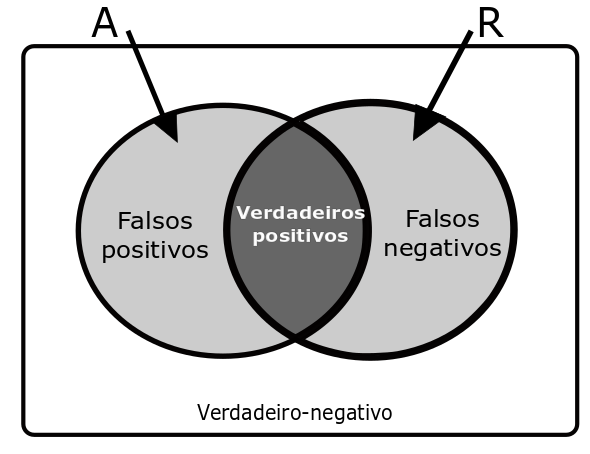
\includegraphics[width=0.9\textwidth]{modelo-monografia-rej-2018/img/DiagramaVenn.png}
    \caption{Diagrama de Venn para Falsos/verdadeiros negativos e positivos}
    \label{fig:Venn}
\end{figure}

\subsection{Análise dos Resultados}
\label{ss:analise}
Após a produção dos resultados e e classificação da situação dos alunos, o passo seguinte do projeto de pesquisa é analisar os resultados para saber se estes foram satisfatório e estão de acordo com o esperado. Para isso serão usados como métrica os índices de Precisão, Acurácia e Cobertura (\textit{Recall}). As formalizações propostas em outras literaturas para essas três métricas são as seguintes:


$Acurácia = \frac{VP+VN}{VP+VN+FP+FN}*100$

$Precisão = \frac{VP}{VP+FP}*100$

$\textit{Recall} = \frac{VP}{VP+FN}*100$

\begin{figure}
    \centering
    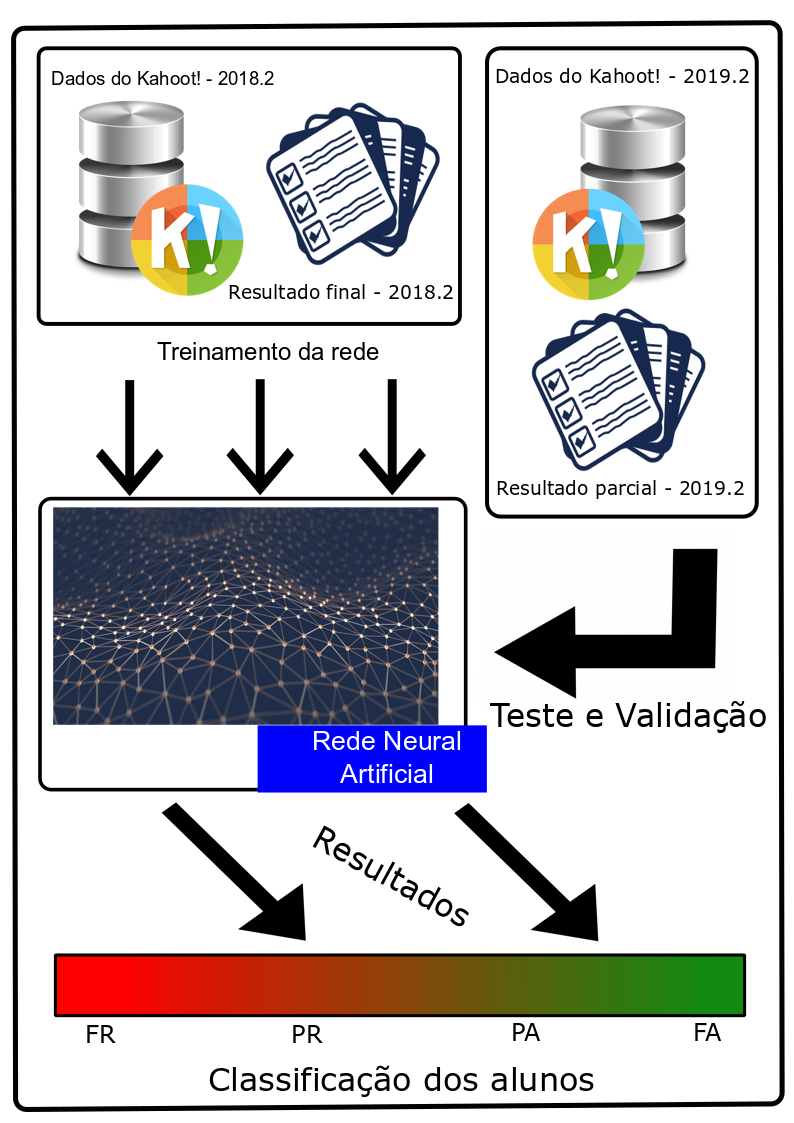
\includegraphics[width=0.5\textwidth]{modelo-monografia-rej-2018/img/ProcessoMetodologico.png}
    \caption{Diagrama esquemático dos processos do projeto de pesquisa}
    \label{fig:processo}
\end{figure}


\section{Estudo de caso}
\label{sec:estudo}
Um estudo de caso é uma investigação empírica que investiga um fenômeno contemporâneo dentro de seu contexto da vida real, especialmente quando os limites entre o fenômeno e o contexto não estão claramente definidos \cite{yin2001planejamento}. Esta investigação enfrenta uma situação tecnicamente única em que haverá muito mais variáveis de interesse do que fonte de dados, e, como resultado, (1) baseia-se em fontes de evidências, com os dados precisando assimilar-se a trabalhos correlatos, e, como outro resultado, (2)beneficia-se do desenvolvimento prévio de proposições teóricas para conduzir a coleta e análise de dados.

\subsection{Descrição do estudo de caso}
Este é um estudo de caso único holístico, utilizando uma estratégia exploratória. A justificativa deste estudo reside no caso revelador que é o uso de RNA na predição de desempenho acadêmico dos alunos em Educação de Computação no Brasil. Os estudos do levantamento bibliográfico concentram-se principalmente em países da América do Norte, Europa e Oceania, como descrito no \autoref{sec:TR}.
Segundo \citeonline{yin2001planejamento}, um estudo de caso contém, em especial, cinco componentes importantes de um projeto de pesquisa que serão descritos a seguir.

%\subsection{Questões do estudo}
Para nortear este estudo de caso, a questão principal levantada foi \textbf{Q1: ``Quais são os resultados ao se utilizar a RNA na previsão de alunos em situação de risco de reprovação em Educação de Computação no contexto Brasileiro?''}

%\subsection{Proposições} \label{sec:HS}
As seguintes proposições foram estabelecidas a fim de serem investigadas. A Proposição 1 \textbf{(P1): ``A precisão da RNA alcançou um nível satisfatório.''}, Proposição 2 \textbf{(P2): ``A acurácia da RNA teve um desempenho satisfatório''} e Proposição 3 \textbf{(P3): ``A cobertura (\textit{Recall}) atingiu um nível satisfatório''}.

\subsection{Unidade de análise e Coleta de Dados}
A unidade de análise do estudo é a turma de 2019.2 da disciplina de Interface Humano-Computador do Bacharelado em Ciência da Computação da Universidade Federal de Jataí, localizada no sudoeste goiano.

A coleta dos dados terá quatro fontes: as respostas dos alunos no Kahoot! de 2018.2 (F1), o resultado final do processo de avaliação somativa dos alunos da turma de 2018.2 (F2), as respostas ao Kahoot! de 2019.2 (F3) e o resultado parcial da avaliação formativa dos alunos da turma de 2019.2 (F4). As duas turmas são da disciplina de Interface Humano-Computador. 

As respostas são dadas pelos alunos, no final de cada aula, às perguntas elaboradas pelo professor que ministra a disciplina, através da ferramenta de tecnologia educacional, ``Kahoot!'', que foi descrita na seção \ref{sec:Kahoot!} e os resultados parciais e finais no processo de avaliação somativa - aprovado ou reprovado - obtidos por esses alunos.

Ao final da disciplina e do processo de avaliação somativa, os alunos alcançam certo resultado - aprovado ou reprovado - que será um dos dados que formará o conjunto que será analisado.

\subsection{Análise dos Dados}
Para demonstrar a ligação entre os dados coletados e as proposições estabelecidas, serão adotadas três métricas, os resultados de \textbf{precisão}, \textbf{Acurácia} e Cobertura (\textit{Recall} obtidos por trabalhos correlatos. Os dados coletados servirão como suporte para a proposição através da métrica adotada. Se os resultados alcançados forem próximos às métricas, podemos dizer que a previsão feita pela RNA atingiu um nível satisfatório. Mais detalhes serão descritos a seguir. Para melhor compreensão, os conceitos de Acurácia e Precisão são importantes de serem explicados e diferenciados e serão na \autoref{dif}. As fórmulas que os descrevem já foram explicitadas na \autoref{ss:analise}.

As métricas usadas serão usadas como suporte para dizer se os resultados alcançados neste projeto satisfizeram as proposições estabelecidas, ou seja, os níveis alcançados foram satisfatórios. Para definir os valores estabelecidos, tomaremos como base os valores obtidos para os atributos de métrica descritos, evidenciando resultados concretos já alcançados. Os trabalhos em questão serão os Trabalhos Relacionados da \autoref{sec:TR}, onde se alcançaram níveis próximos ao que será estabelecido para este, que terá uma margem de consideração. Formalmente, podemos dizer que as métricas que servirão de base, serão:

$Acurácia = \left \{ x | x >= 70\% \right \}$

$Precisão = \left \{ y | y >= 75\% \right \}$

;$Recall = \left \{ z | z >= 70\% \right \}$
\subsubsection{Diferença entre Precisão e Acurácia} \label{dif}

\textbf{Precisão} se define como a proximidade entre os valores obtidos pela repetição do processo de mensuração. Quanto menor é a diferença destes valores, melhor é a precisão. \textbf{Acurácia} se define como a proximidade da medida em relação ao verdadeiro valor, um valor definido, que se deseja obter. Quanto mais próximo do valor real, melhor é a acurácia. A \autoref{fig:PrecAcur} esclarece isso de maneira bem didática.

\begin{figure}
    \centering
    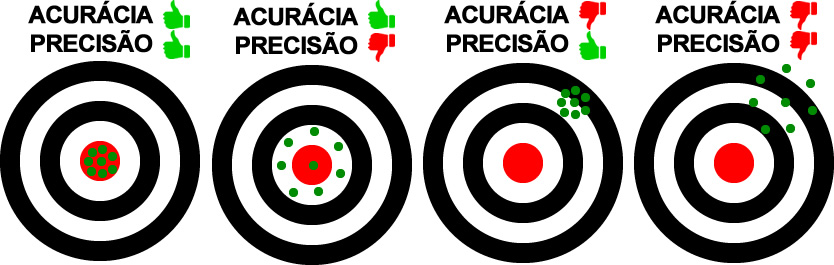
\includegraphics[width=0.9\textwidth]{modelo-monografia-rej-2018/img/PrecisaoAcuracia.jpg}
    \caption{Diferença entre Acurácia e Precisão}
    \label{fig:PrecAcur}
\end{figure}

\section{Classificação da pesquisa}
\label{sec:classif}
A classificação desse projeto de pesquisa pode ser feito em termos de gêneros da mesma. Estes gêneros dizem respeito à natureza, os objetivos, os procedimentos, o objeto e à forma de abordagem desta.

\subsection{Gêneros de Pesquisa}

{\color{red} COLOCAR FRASE}

\subsubsection{Quanto à natureza}
Empírica, pois a pesquisa dedica-se recolher dados diretamente da realidade do objeto de estudo, mensurar a realidade, formular observações e propor transformações do mesmo enquanto objeto de investigação, mas não intervem de forma concreta no ambiente durante o trajeto da pesquisa.

\subsubsection{Quanto aos objetivos}
Pesquisa exploratória: Apesar de haverem pesquisas em relação à métodos para a predição dos resultados do processo de avaliação somativa --- aprovado ou reprovado ---, há a necessidade de se relatar casos no Brasil, que ocorram experimentos da aplicação desses métodos no processo de avaliação de aprendizagem, identificando alunos em situação de risco.

\subsubsection{Quanto aos procedimentos}
Pesquisa de Campo: Todos os procedimentos que serão usados nesta pesquisa serão derivados de coletas de dados realizadas em fontes diretas. Desta forma, esta pesquisa quantos aos procedimentos é de campo, pois baseia-se em dados coletados no local da ocorrência dos fatos.

\subsubsection{Quanto ao objeto}
Pesquisa de campo: O principal objeto desta pesquisa é justamente a identificação prévia de alunos em risco de reprovação e o uso de Redes Neurais Artificiais como método preditivo. O conceito sobre o objeto, o problema relacionado ao mesmo, assim como a justificativa, são oriundos de uma coleta de dados realizada em local, tornando esta pesquisa de campo quanto aos objetos.

\subsubsection{Quanto à forma de abordagem}
Pesquisa quantitativa: Serão coletadas as respostas dadas pelos alunos, analisando os dados gerados, com o modelo de Rede Neural criado, e produzindo, assim, uma saída classificada.